\section*{Fourth Design}
Hand calculations reveal that due to the negative and positive constant operands to the multipliers, it is impossible to cause an underflow or overflow condition to occur. The previous ripple carry adder module handled overflow/underflow, however, in an effort to reduce adder delay, the optimized Verilog library adder is used in this iteration of design. It is hoped that this design will allow the pipelined multipliers to be leveraged. 
\subsection*{Final Verilog Code Iteration}
Due to time constraints the design process ends with this code for the filter. 

\subsection*{Using Optimized Adders}
module add2\_16(a, b, cin, sum, cout);\\*
  output reg [15:0] sum;\\*
  output reg cout;\\*
  input [15:0] a;\\*
  input [15:0] b;\\*
  input cin;\\*
\\*
  always @(a, b, cin)\\*
    {cout, sum} = a + b + cin;\\*
endmodule\\*


\subsection*{Fourth Design Timing Analysis}

% Table generated by Excel2LaTeX from sheet 'Sheet1'
\begin{table}[bh]
\caption{Xilinx Timing Report}
\begin{tabular}{c|c}
\centering
           & Timing in (ns) \\
\hline
     Delay &   11.445  \\

Requrement &    100.000 \\

Data Path Delay & 11.369  \\
\end{tabular}  
\label{tab:timing4}
\end{table}

According to Table \ref{tab:timing4}, the maximum clock frequency for the this design has been calculated to be approximately: 87.4 MHz. This result proves that using the optimized library adder greatly reduces the critical path delay and increases clock frequency by over a third. Refer to Figure \ref{subfig:output4-b} to review the filter output. The block diagram for this design is the same as the third iteration, but is included for consistency. 

\begin{figure}[htp]
  \begin{center}
    \subfigure[Functional block diagram]{\label{subfig:block4-a}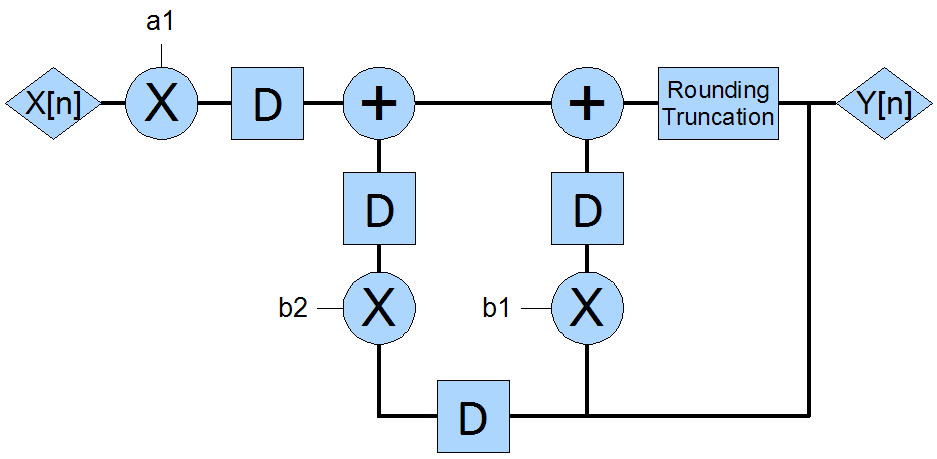
\includegraphics[scale=0.30]{block_three.png}}
    \subfigure[Input/Output comparison]{\label{subfig:output4-b}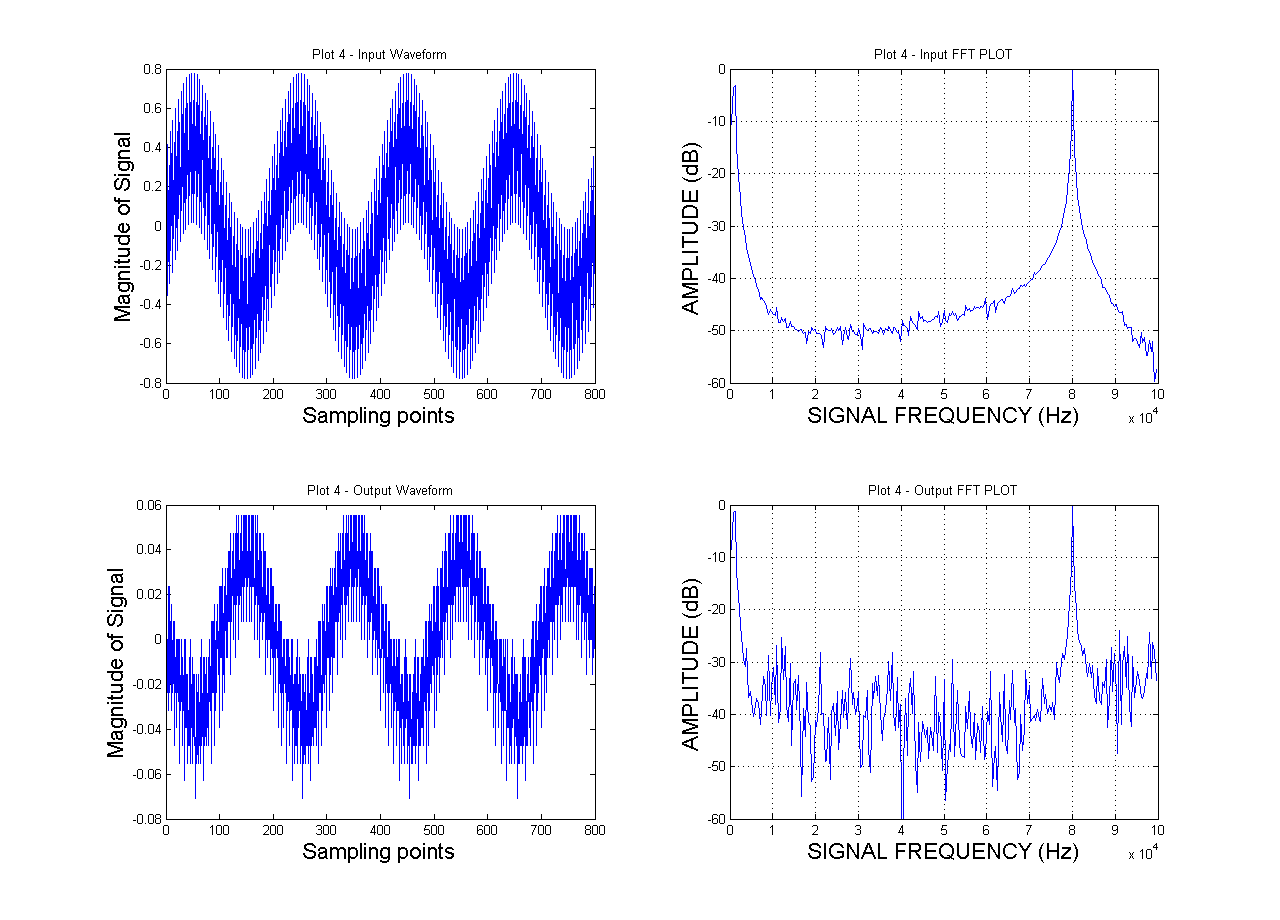
\includegraphics[scale=0.30]{plot4.png}} \\*
  \end{center}
  \caption{Second Design Results}
  \label{fig:design4_results}
\end{figure}

\subsection*{Final Verilog Code Iteration}
As a recap, changes that lead to this final design include: rounding before truncation (Listing \ref{lst:filt_code}), pipelined multipliers (Listing \ref{lst:mult8_code}) to reduce path delay, and library based adders (Listing \ref{lst:adder16_code}) to reduce the high delay incurred by the ripple carry. The Matlab code was modified to print both the input and output simultaneously to hasten the simulation and testing process. Refer to Listing \ref{lst:plot_code} to review the changes to the Matlab code.
\\*
\lstset{language=verilog}
\lstinputlisting[caption=Final Filter Module, label=lst:filt_code]{plot4code/projfilt.v}
\lstinputlisting[caption=Sixteen Bit Adder, label=lst:adder16_code]{plot4code/add2_16.v}
\lstinputlisting[caption=Eight Bit Truncation Adder, label=lst:adder8_code]{plot4code/add2_8.v}
\lstinputlisting[caption=Eight Bit Multiplier, label=lst:mult8_code]{plot4code/mult8.v}
\lstinputlisting[caption=Eight Bit Register, label=lst:reg8_code]{plot4code/reg8.v}
\lstinputlisting[caption=Matlab Code, label=lst:test_code]{plot4code/filter_test.v}
\lstset{language=matlab}
\lstinputlisting[caption=Firt Iteration, label=lst:plot_code]{matlab/plot_filter.m}
